%---------- Inleiding ---------------------------------------------------------

\section{Introductie}%
\label{sec:introductie}

De onderzoeksvraag werd aangeboden door het bedrijf IntelliProve. IntelliProve biedt online gezondheidsoplossingen, een software die in staat is om binnen enkele seconden nauwkeurig gezondheidsparameters te bepalen, gebaseerd op een optische meting van het gezicht.  
Het doel van de bachelorproef is het ontwikkelen en implementeren van een robuust systeem voor het schatten van de leeftijd en het geslacht van personen op basis van gezichtsfoto's, met behulp van machine learning-technieken. 
Dit project is van bijzonder belang voor het verbeteren van de beoordeling van de geestelijke gezondheidszorg door middel van camera-gebaseerde gezondheidsmetingen. Het onderzoek beoogt bij te dragen aan de vooruitgang op dit gebied door gebruik te maken van geavanceerde algoritmen om leeftijd en geslacht nauwkeurig te voorspellen aan de hand van gezichtsbeelden.  
De literatuurstudie biedt een inzicht in facial analysis, de bestaande machine learning modellen en hun functionaliteiten. De proof-of-concept zal bestaan uit het ontwikkelen van een machine learning pipeline dat in staat is om leeftijd en geslacht te voorspellen op basis van bestaande datasets. De pipeline omvat verschillende image preprocessing technieken om de dataset voor te bereiden op de modeltraining. Om betrouwbaarheid en accuracy te garanderen, worden de modellen verfijnd en geoptimaliseerd om de hoogst mogelijke nauwkeurigheid te bereiken bij het schatten van leeftijd en geslacht.

\section{Stand van zaken}
\label{sec:stand-van-zaken}

Gezichtsanalyse bestaat uit het definiëren van menselijke gezichten in real-time, met behulp van computeralgoritmen en machine learning-technieken. Voor computersystemen bevat een gezichtsbeeld details zoals leeftijd, geslacht, stemming, ras, et cetera. 
Gezichtsanalyse omvat dan ook het lokaliseren en kwantificeren van gezichtskenmerken in een afbeelding. Vervolgens wordt het gezichtsbeeld geanalyseerd voor het extraheren van kenmerken \autocite{Sanil2023}. Gezichtsanalyse speelt dan ook een grote rol in real-world applicaties, zoals animatie, identiteitsverificatie, medische diagnose, et cetera. Ondanks het bestaande onderzoekswerk over dit onderwerp, is gezichtsanalyse nog steeds een lastige taak vanwege verschillende factoren zoals veranderingen in hoek, gezichtsuitdrukkingen en achtergrond \autocite{Siddiqi2022}. 
Volgens onderzoek van \textcite{BasystiukMR23} is beeldherkenning een simpele procedure die slechts uit 3 stappen bestaat. 
\begin{enumerate}
    \item Preprocessing: We voegen filters toe aan de afbeelding om het geschikter te maken voor herkenning.
    \item Feature Extractie: We identificeren belangrijke data en behouden deze om mee verder te werken. Dit wordt verder besproken in \ref{sub:gezichtsdetectie}
    \item Classificatie: het analyseren en identificeren van de  data na de feature extractie.
\end{enumerate}

\subsection{Gezichtsdetectie}
\label{sub:gezichtsdetectie}
Gezichtsdetectie is de eerste stap in het bepalen van de gezichtsfeatures. Deze features zijn de interessante delen van het gezicht, bijvoorbeeld ogen, neus en mond en worden ook wel eens landmarks genoemd \autocite{Coppens2018}. In dit onderzoek worden 3 gezichtsdetectieservices aangeraden: Microsoft Face API, Face++ en Kairos. Deze zijn alle 3 ook geschikt om geslacht en leeftijd te voorspellen. Er wordt met 3 services tegelijk gewerkt om elkaars beperkingen op te vangen. 
In het onderzoek van \textcite{Sanil2023} worden de landmarks berekend op 2 verschillende methoden: Euclidische afstand en Geodetische afstand. 
\textcite{Sanil2023} stelt 468 landmarks visueel voor, in plaats van 68, om de accuracy te verbeteren. Dit door gebruik te maken van de Mediapipe library (\textcite{Zubair2021}) te gebruiken. Op figuur (~\ref{fig:landmarks}) staan de belangrijkste anthropometrische landmarks aangeduid. Het is noodzakelijk om de belangrijkste features te identificeren die kunnen leiden tot het correct voorspellen van de leeftijd of het geslacht. Om de leeftijd te voorspellen kunnen we bijvoorbeeld de rimpels op de gezichtsfoto analyseren \autocite{Kwon1994}. 
\begin{figure}
    \centering
    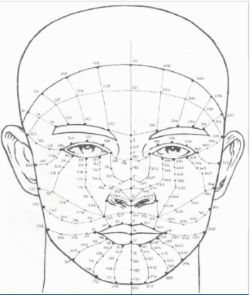
\includegraphics[width=\columnwidth]{graphics/faciallandmarks.png}
    \caption{\label{fig:landmarks}De belangrijkste anthropometrische landmarks\autocite{Sanil2023}.}
\end{figure}

\subsubsection{Normalisatie}
In onderzoek van \autocite{Chen2011} werden de gezichtsafbeeldingen genormaliseerd voor de feature extraction plaats vond. De geometrie van de afbeeldingen kan worden genormaliseerd op basis van de gedetecteerde features, zoals oog of mond coördinatie. Er wordt een mask gebruikt om de pixels die niet in de ovaal van de typische gezichtsregio zitten worden verwijdert. Dit gaat dan over bijvoorbeeld over haar en hemdkragen. Zo blijven enkel de belangrijkste features van het gezicht over. Figuur (~\ref{fig:beforenormalisation}) geeft een voorbeeld van een dataset met gezichtsfoto's. In figuur {~\ref{fig:afternormalisation}} worden deze afbeeldingen genormaliseerd, waardoor er minder variaties overblijven in de afbeeldingen en we bijvoorbeeld al geen achtergrond meer overhouden.
\begin{figure}
    \centering
    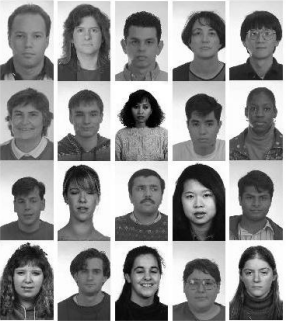
\includegraphics[width=\columnwidth]{graphics/beforenorm.PNG}
    \caption{\label{fig:beforenormalisation}Gezichtsafbeeldingen voor normalisatie\autocite{Chen2011}.}
\end{figure}
\begin{figure}
    \centering
    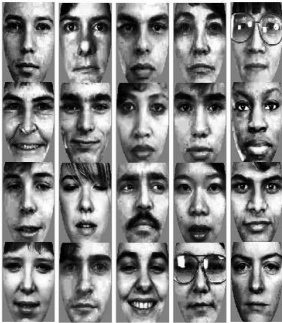
\includegraphics[width=\columnwidth]{graphics/afternorm.PNG}
    \caption{\label{fig:afternormalisation}Gezichtsafbeeldingen na het toepassen van normalisatie\autocite{Chen2011}.}
\end{figure}  

\subsection{Bestaande uitdagingen}
Ondanks het onderzoekwerk, heersen er nog vele uitdagingen op het vlak van gezichtsanalyse. Deze uitdagingen zijn het gevolg van verschillende factoren zoals gezichtsuitdrukkingen, ruis, belichting, et cetera. Om de nauwkeruigheid van de gezichtsherkenning te verbeteren, is het belangrijk om taken van de gezichtsanalyse met elkaar te correleren. Het is bijvoorbeeld zeer waarschijnlijk dat mannen een baard of snor kunnen hebben, maar vrouwen en kinderen niet \autocite{Siddiqi2022}.  Ook is het detecteren van de locatie waar de gezichten zich bevinden op de afbeelding een uitdaging. Dit wordt vaak meegenomen in de preprocessing stap van het analysesysteem \autocite{Jiang2008}. 
De problemen situeren zich niet enkel op het vlak van de afbeelding, maar ook bij de machine learning modellen. Eén van de grootste problemen hierbij is overfitting. Dit gebeurt wanneer het algoritme te veel getraind wordt waardoor het te hard lijkt op de trainingsdata. Hierdoor zal het systeem falen wanneer er nieuwe data moet worden geclassificeerd \autocite{Coppens2018}.

\subsection{Bestaande Machine-Learning technieken}
Uit onderzoek van \textcite{Sanil2023} bleek dat Extreme gradient boosting de beste resultaten gaf, met een accuracy van 78\%, gevolgd door Adaptive Boosting (77\%) en Random Forest (75\%). Onderzoek van \autocite{Khan2017} gebruikt dan weer een Ensemble systeem. Een set van 30 Lineaire Discriminant Analyse (LDA) dienen als basis classifiers en dragen bij tot het ensemble. Het ensemble gebruikt de gecombineerde classificatiecapaciteiten van de base classificiers, zo verbeteren we de algehele prestaties. De volledige pipeline voor de gezichtsanalyse vinden we in figuur (~\ref{fig:ensemble}). 
\begin{figure}
    \centering
    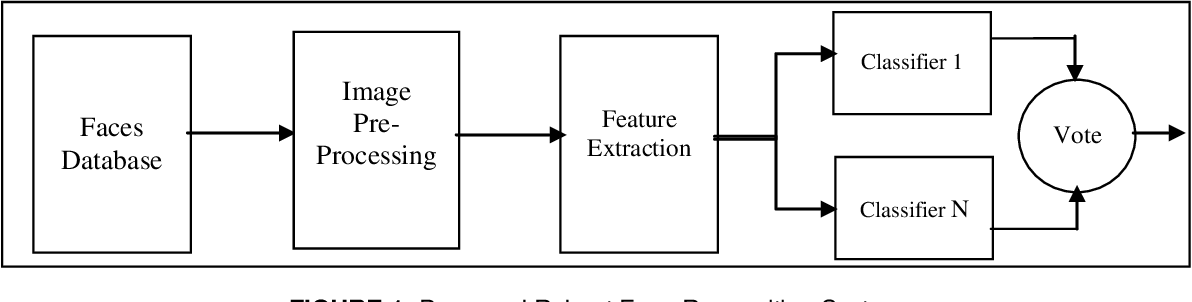
\includegraphics[width=\columnwidth]{graphics/ensemble.png}
    \caption{\label{fig:ensemble}Robuust Gezichtsherkenning systeem\autocite{Khan2017}.}
\end{figure}

\subsubsection{Extreme Gradient Boost}
\label{subsub:xgboost}
Extreme Gradient Boost, ofwel XGBoost, is een supervised learning model, waar trainingdata, met meerdere features, x\textsubscript{i} wordt gebruikt om target waarde y\textsubscript{i} te voorspellen \autocite{XGBoost2023}. Uit onderzoek van \autocite{Chen2023}, waarbij vermoeidheid werd voorspeld op basis van gezichtsafbeeldingen met XGBoost wordt een boom aangemaakt op basis van de geleverde features. Dit model gaf een hoge accuracy en is minder gevoelig voor noise. 

\subsubsection{Adaptive Boosting}
\label{subsub:adaboost}
De Adaptive Boost, of AdaBoost, is typisch een classificatie tussen twee klassen. Om het herkenningsprobleem met meerdere klassen op te lossen op te lossen, kan een majority voting (MV) strategie worden gebruikt om alle paarsgewijze classificatieresultaten te combineren. Hierbij kiezen we de meest voorkomende klasse als voorspelling. AdaBoost is een adaptief algoritme om een reeks classificeerders te boosten, in die zin dat de gewichten dynamisch worden bijgewerkt op basis van de fouten in eerdere leerresultaten \autocite{Guo2001}.

\subsubsection{Random Forest Classifier}
\label{subsub:randomforest}
Random forests zijn verzamelingen decision trees die elk getraind zijn op een willekeurig gekozen deelverzameling van de beschikbare data. Deze decision trees worden willekeruig door de trainingsvoorbeelden die aan elke boom worden gegeven,  maar ook door een willekeurige subset van tests die beschikbaar zijn voor optimalisatie op elke node \autocite{Fanelli2012}. 
Een voorbeeld voor het gebruik van Random Forest in gezichtsanalyse is figuur((~\ref{fig:randomforest}))). Hierbij wordt een boom getoond voor het  schatten van de houding van het hoofd. 
\begin{figure}
    \centering
    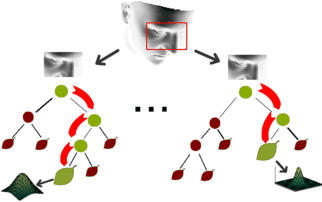
\includegraphics[width=\columnwidth]{graphics/headposition.png}
    \caption{\label{fig:randomforest}Voorbeeld van een random forest voor het schatten van de houding van het hoofd\autocite{Fanelli2012}.}
\end{figure}

% Voor literatuurverwijzingen zijn er twee belangrijke commando's:
% \autocite{KEY} => (Auteur, jaartal) Gebruik dit als de naam van de auteur
%   geen onderdeel is van de zin.
% \textcite{KEY} => Auteur (jaartal)  Gebruik dit als de auteursnaam wel een
%   functie heeft in de zin (bv. ``Uit onderzoek door Doll & Hill (1954) bleek
%   ...'')


%---------- Methodologie ------------------------------------------------------
\section{Methodologie}%
\label{sec:methodologie}

\subsection{Requirements}
\label{sub:requirements}
In de eerste week wordt nagevraagd aan belanghebbenden van IntelliProve aan welke criteria de modellen moeten voldoen. Alle data (gezichtsfoto's) worden verzameld. Er wordt onder andere nagegaan over welke functionaliteiten de modellen moeten beschikken en wat de verwachte prestatievereisten zijn. 
Als resultaat verwerven we een lijst van alle functionele en niet-functionele requirements, geordend volgens belang. 

\subsection{Literatuurstudie}
\label{sub:literatuurstudie}
De literatuurstudie omvat een diepgaande verkenning van facial analysis technieken en machine learning modellen. 
Deze fase biedt inzicht in de verschillende methoden voor het extraheren van gezichtskenmerken en image preprocessing technieken, specifiek met betrekking tot het schatten van leeftijd en geslacht.
Het doel is om kennis uit bestaand onderzoek te vergaren om effectieve methodologieën te identificeren in de huidige benaderingen van facial analysis. 
Het eindresultaat van deze fase, die 3 weken duurt, is een samenvatting van de belangrijkste bevindingen uit de literatuurstudie, die als basis zal dienen voor de proof-of-concept.
\subsection{Proof-of-concept}
\label{sub:proof-of-concept}
Deze fase start met het verzamelen en analyseren van de datasets. Technieken zoals normalisatie en scaling van de features, feature-extractie en data augmentation worden gebruikt om de dataset voor te bereiden op modeltraining.
Vervolgens worden verschillende machine learning algoritmen geselecteerd op basis van de bevindingen uit de literatuurstudie. De modellen worden getraind en geëvalueerd op basis van de vooropgestelde requirements. 
De pipeline wordt beoordeeld op betrouwbaarheid en precisie op basis van de opgestelde requirements. Metrieken zoals accuracy, precision, recall, F1-score en ROC-curves worden gebruikt om de modellen te evalueren.
Er worden cross-validatie technieken gebruikt om de robuustheid van de modellen en de generalisatie van nieuwe data te testen. 
Deze fase vereist dan ook veel tijd en zal 6 weken duren. Het resultaat van deze fase is een proof-of-concept die bestaat uit een machine learning pipeline, die stappen voor het preprocessen van gegevens en getrainde modellen integreert voor het schatten van leeftijd en geslacht op basis van gezichtsfoto's.

\subsection{conclusie}
\label{sub:conclusie}
In de conclusiefase worden de resultaten van de evaluatie grondig geanalyseerd. De prestaties van de ontwikkelde modellen worden beoordeeld, waarbij hun sterke punten en beperkingen worden benadrukt. Het belang van een nauwkeurige schatting van leeftijd en geslacht bij de beoordeling van de geestelijke gezondheid en de implicaties voor de gezondheidszorg worden besproken. Er worden aanbevelingen gedaan voor mogelijke verbeteringen of toekomstige onderzoeksrichtingen op basis van de bevindingen en beperkingen van het project.
\subsection{Afwerken scriptie}
\label{sub:afwerken_scriptie}
De laatste fase, die 2 weken duurt, omvat het afwerken van de bachelorproef. Dit is het eindresultaat van het geleverde onderzoek met een proof-of-concept die zal worden ingediend. 


%---------- Verwachte resultaten ----------------------------------------------
\section{Verwacht resultaat, conclusie}%
\label{sec:verwachte_resultaten}

Hier beschrijf je welke resultaten je verwacht. Als je metingen en simulaties uitvoert, kan je hier al mock-ups maken van de grafieken samen met de verwachte conclusies. Benoem zeker al je assen en de onderdelen van de grafiek die je gaat gebruiken. Dit zorgt ervoor dat je concreet weet welk soort data je moet verzamelen en hoe je die moet meten.

Wat heeft de doelgroep van je onderzoek aan het resultaat? Op welke manier zorgt jouw bachelorproef voor een meerwaarde?

Hier beschrijf je wat je verwacht uit je onderzoek, met de motivatie waarom. Het is \textbf{niet} erg indien uit je onderzoek andere resultaten en conclusies vloeien dan dat je hier beschrijft: het is dan juist interessant om te onderzoeken waarom jouw hypothesen niet overeenkomen met de resultaten.

